\subsubsection{Pregled uplata}
\label{subsubsec:vozni park}
\begin{itemize}
  \item \textbf{Kratak opis}: Računovođa vodi računa o uplatama kandidata i može da obriše ili izmeni uplatu.

  \item \textbf{Učesnici}:
    \begin{itemize}
    \item Računovođa - korisnik sistema koji ima uvid o uplatama kandidata.
    \end{itemize}
  \item \textbf{Preduslovi}:
    \begin{itemize}
    \item  Sistem je u funkciji.
    \end{itemize}
  \item \textbf{Postuslovi}:
      \begin{itemize}
      \item  Računovođa ima evidenciju o svim uplatama.
      \end{itemize}
  \item \textbf{Osnovni tok}:
      \begin{enumerate}
        \item Računovođa otvara stranicu za logovanje.
        \item Računovođa unosi ID i lozinku.
        \item Klikom na dugme "Prijavi se" računovođa se prijavljuje na svoj profil.
        \item Klikom na polje "Izveštaji" otvara se opadajući meni.
        \item Klikom na polje "Pregled uplata" računovođa dobija informacije o svim uplatama.
      \end{enumerate}

  \item \textbf{Alternativni tokovi}:
      \begin{itemize}
        \item A1. \textbf{Računovođa unosi pogrešan ID ili lozinku:}
        Ukoliko u koraku 2 računovođa unese pogrešan ID ili lozinku, ne može da se prijavi na svoj profil i proces se nastavlja u koraku 1.
      \end{itemize}

\end{itemize}

\begin{figure}[H]
  \begin{center}
      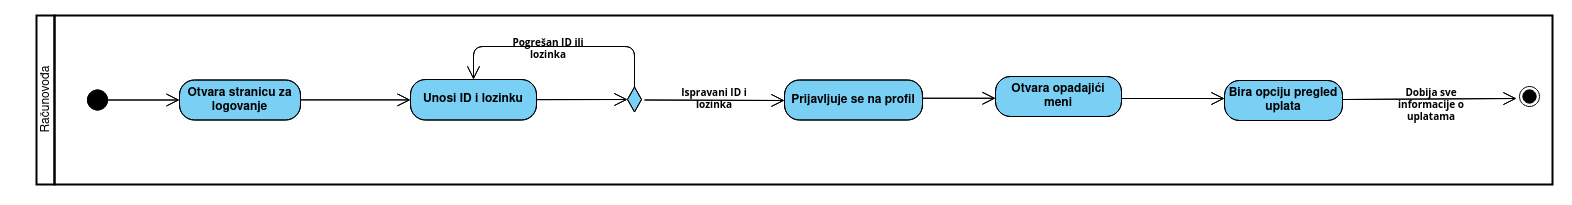
\includegraphics[width=170mm, height=70mm]{Diagrams/dijagram_aktivnosti_pregled_uplata.png}
  \end{center}
  \caption {Dijagram aktivnosti - Pregled uplata}
  \label{activity_pregled_uplata}

\end{figure}
